\documentclass[14pt]{beamer}

\mode<presentation> {
\usetheme{Madrid}

% To remove the navigation symbols from the bottom of all slides uncomment next line
\setbeamertemplate{navigation symbols}{} 
\date{}
\title{}
\author{}

%to get rid of footer entirely uncomment next line
\setbeamertemplate{footline}{}
}


\usepackage{geometry}
\usepackage{multirow}
\usepackage{adjustbox}
\usepackage{multicol}
\setlength{\columnsep}{0.1cm}



\usepackage{tikz}
\usetikzlibrary{shapes,backgrounds}

\usepackage{bbding}
\usepackage{rotating}
\usepackage{xcolor}


%\usepackage{tkz-berge} %cool grid
\usepackage{pgfplots} %pics

\usepackage{graphicx} % Allows including images
\usepackage{booktabs} % Allows the use of \toprule, \midrule and \bottomrule in tables
\usepackage{mathtools}

\newcommand {\DS} [1] {${\displaystyle #1}$}
\newcommand {\R}{\mathbb{R}}
\newcommand {\Z}{\mathbb{Z}}
\newcommand {\N}{\mathbb{N}}
\newcommand{\e}{\varepsilon}

\newcommand{\p}{\pause}

% simple environrment for enumerate, easier to read
\setbeamertemplate{enumerate items}[default]

%%%%%%%%%%%%%%%%%%%%%%

% to use colours easily
\definecolor{miverde}{rgb}{0.7, .5, 0.7}
\newcommand{\azul}[1]{{\color{blue} #1}}
\newcommand{\rojo}[1]{{\color{red} #1}}
\newcommand{\verde}[1]{{\color{miverde} #1}}
 
% box in red and blue in math and outside of math
\newcommand{\cajar}[1]{\boxed{\mbox{\rojo{ #1}}}}
\newcommand{\majar}[1]{\boxed{\rojo{ #1}}}
\newcommand{\cajab}[1]{\boxed{\mbox{\azul{ #1}}}}
\newcommand{\majab}[1]{\boxed{\azul{ #1}}}
 
\newcommand{\setsize}[1]{\fontsize{#1}{#1}\selectfont} %allows you to change the font size. The default size of this document is 14. To change the font size of the whole slide, place this at the beginning of the slide. To change the size of only a portion of the text to size 12, you can do the following { \setsize{12} Your text. }.

\setbeamerfont{frametitle}{size=\setsize{15}}
\setbeamerfont{block title}{size=\setsize{14}}

\newcommand{\smallerfont}{\setsize{13}} %place this at the beginning of a slide to set the font size of the entire slide to 13.

%===========================
% For UNIT 2 specifically:

\newcommand{\floor}[1]{\lfloor #1 \rfloor}


\setbeamertemplate{enumerate items}{(\Alph{enumi})}


%===================================================
\begin{document}
%===================================================

\begin{frame}
\frametitle{MAT137 Lecture 7 --- Absolute Values}
	{\bf Warmup:}
\vfill

	You want to show ``$\exists n\in \mathbb N\text{ s.t. }n^2=4$''. Which proofs below
	are correct/incorrect?
	\begin{multicols}{2}

		\begin{enumerate}
		

			\item Let $n=2$. Then, $n\in \mathbb N$ and $n^2=4$.


			\item 		Let $n\in \mathbb N$. Take $n=2$. Then $n^2=4$.

		\columnbreak

	\item 		Let $n\in\mathbb N$. Assume $n=2$. Then $n^2=4$.


		
	\item	Take $n=4$. Then $n\in \mathbb N$ and $n^2=4$.

		\end{enumerate}

	\end{multicols}

	\vfill
	{\bf Before next class:}
		\begin{itemize} \normalsize
			\item {\bf Watch videos 2.1, 2.2, 2.3 }
		\end{itemize}
	\vfill

\end{frame}


%------------------------------
\begin{frame}
\frametitle{Variations on induction}

Let $S_n$ be a statement depending on a positive integer $n$.

\vfill  

	What conclusions can you draw in each of the following cases? (I.e., for which $n$ do you
	know that $S_n$ is true?)

\vfill 

\begin{multicols}{2}
\begin{enumerate}
\item  We have proven:
	\begin{itemize}
		\item   $S_3$ 
		\item  \DS{\forall n \geq 1, \; S_{n}  \implies S_{n+1} }
	\end{itemize}	
\item  We have proven:
	\begin{itemize}
		\item  $S_1$ 
		\item  \DS{\forall n \geq 3, \; S_{n} \implies S_{n+1} }
	\end{itemize}	
\item  We have proven:
	\begin{itemize}
		\item  $S_1$ 
		\item  \DS{\forall n \geq 1, \; S_{n} \implies S_{n+3} }
	\end{itemize}	
\item  We have proven:
	\begin{itemize}
		\item  $S_1$ 
		\item  \DS{\forall n \geq 1, \; S_{n+1}  \implies S_{n} }
	\end{itemize}	
\end{enumerate}	
\end{multicols}

\vfill

\end{frame}


%-----------------------------
\begin{frame}
\frametitle{Variations on induction 2}

We want to prove  
	$$\forall n \geq 1, \; S_n $$
	
\vfill

So far we have proven
	\begin{itemize}
		\item  $S_1$ 
		\item  \DS{\forall n \geq 1, \; S_n \implies S_{n+3}.}
	\end{itemize}	

\vfill	

What else do we need to do?

\end{frame}

%----------------------------
\begin{frame}
\frametitle{What is wrong with this proof by induction?}
\smallerfont

\vspace{-1.5mm}
\begin{theorem}
$\forall N \geq 1$, every set of $N$ students in MAT137 will get the same grade.
\end{theorem} \p
\vspace{-1mm}

\begin{proof}
\begin{itemize} 
	\item  {\bf Base case.}  It is clearly true for $N=1$.
	\item  {\bf Induction step.}  \\
		Assume it is true for $N$.  I'll show it is true for $N+1$. \\
		Take a set of $N+1$ students.  By induction hypothesis:
			\begin{itemize}
				\item  The first $N$ students get the same grade.
				\item  The last $N$ students get the same grade.
			\end{itemize}
			$$
				\mathrlap{\overbrace{\phantom{\bullet \quad \bullet \quad \cdots \quad \bullet \quad \bullet }}^{\text{Same grade}}}
				\bullet \quad \underbrace{\bullet \quad \bullet \quad \cdots \quad \bullet \quad \bullet}_{\text{Same grade}}
			$$
		Hence the $N+1$ students all get the same grade.
\end{itemize}
\end{proof}

\end{frame}
%----------------------------
\begin{frame}
\frametitle{What is wrong with this proof by induction?}

For every $N \geq 1$, let
	\begin{center}
	\begin{tabular}{rcc}
		\DS{S_N} =  & ``every set of $N$ students in MAT137 \\ & will get the same grade"
	\end{tabular}
	\end{center}

\vfill 

What did we actually prove in the previous page?

	\begin{itemize}
		\item  $S_1$ \, ?
		\item  \DS{\forall N \geq 1}, \, \DS{S_N \implies S_{N+1}} \, ?
	\end{itemize}

\vfill 
\end{frame}


%-----------------------------
\begin{frame}
\frametitle{Properties of absolute value}


Let $a, b \in \mathbb{R}$.  
	Are the following conclusions correct?

	\vfill
\begin{enumerate}
	\item  \DS{ |ab|  = |a| |b|}
	\item  \DS{ |a + b | = |a| + |b|}
\end{enumerate}

\vfill

If any of the conclusions is wrong, fix it.


\end{frame}

%-----------------------------
\begin{frame}
\frametitle{Properties of inequalities}

Let $a, b, c \in \mathbb{R}$.  \\
 Assume $a < b$.  
	Are the following conclusions correct?

\begin{enumerate}
\begin{multicols}{2}
	\item  \DS{a + c < b + c}  
	
	\
	\item  \DS{a-  c < b - c}  
	
	\
	\item  \DS{ac < bc}
	
	\
	\item  \DS{a^2 < b^2}
	
	\
	\item  \DS{\frac{1}{a} < \frac{1}{b}}	
	
	\
	\item  \DS{\sin a<\sin b}	
\end{multicols}
\end{enumerate}

\vfill
If any of the conclusions is wrong, fix it.

\end{frame}

%-----------------------------
\begin{frame}
\frametitle{Sets described by distance}


Let $a \in \R$.  Let $\delta >0$.  \\
Describe the following sets using interval notation.

\begin{enumerate}
	\item  \DS{A = \{x \in \R \; : \; |x| < \delta\} }
	\item  \DS{B = \{x \in \R \; : \; |x| > \delta\} }
	\item  \DS{C = \{x \in \R \; : \; |x-a| < \delta\} }
	\item  \DS{D = \{x \in \R \; : \; 0 < |x-a| < \delta\} }
\end{enumerate}


\end{frame}
%-----------------------------
\begin{frame}
\frametitle{Implications}

Find \emph{all} positive values of $X$, $Y$, and $Z$ which make the following implications true.

\vfill
\begin{enumerate}
	\item  \DS{| t-3 | <  1  \implies |2t-6| < X}
	
		\

	\item   \DS{|t-3| < Y \implies |2t-6| < 1}

		\

	\item  \DS{|t-3| < 1 \implies |t+5| < Z}
\end{enumerate}
\vfill

\end{frame}


\begin{frame}
\frametitle{MAT137 Lecture 8 --- Limits}
	\vfill
	{\bf Before next class:}
		\begin{itemize} \normalsize
			\item {\bf Watch videos 2.5, 2.6 }
		\end{itemize}
	\vfill

\end{frame}


%-----------------------------
\begin{frame}
\frametitle{Limits from a graph}

\begin{columns}[c]

\column{.65\textwidth}

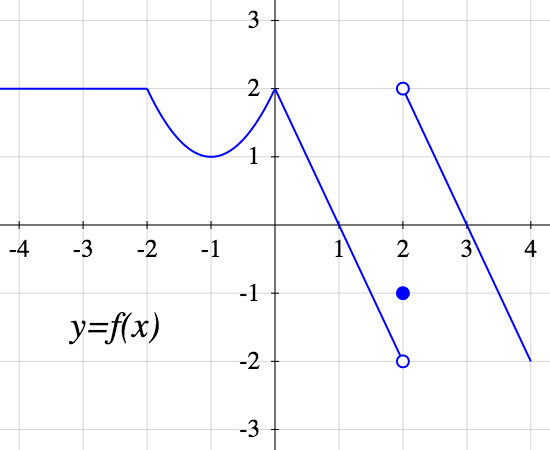
\includegraphics[scale=.4]{G1}

\column{.33\textwidth}
Find the value of 
\begin{enumerate}
	\item  \DS{\lim_{x \to 2} f(x)}
	\item  \DS{\lim_{x \to 0} f(f(x))}
		\p
	\item  \DS{\lim_{x \to 2} \left[ f(x) \right]^2}
	\item \DS{\lim_{x \to 0} f(2 \cos x)}
\end{enumerate}
\end{columns}

\end{frame}
%-----------------------
\begin{frame}[t]
\frametitle{Floor}

Given a real number $x$, we defined the \emph{floor of $x$}, denoted by $\floor{x}$, as the largest integer smaller than or equal to $x$.  For example:
	$$
	 	\floor{\pi} = 3, \quad \quad \floor{7}=7, \quad \quad \floor{-0.5}=-1.
	$$
Sketch the graph of \DS{y = \floor{x}}.  Then compute:	 	
\begin{multicols}{2}
		\begin{enumerate}
			\item \DS{\lim_{x \to 0^+} \floor{x}}
			\item \DS{\lim_{x \to 0^-} \floor{x}}
			\item \DS{\lim_{x \to 0} \; \floor{x}}
			\item \DS{\lim_{x \to 0} \; \floor{x^2}}
		\end{enumerate}
\end{multicols}

\end{frame}
%-----------------------------
\begin{frame}
\frametitle{More limits from a graph}

\begin{columns}[c]

\column{.65\textwidth}

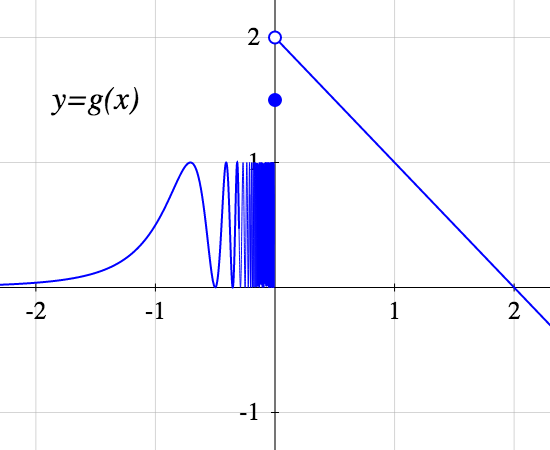
\includegraphics[scale=.4]{G2}

\column{.33\textwidth}
Find the value of 
\begin{enumerate}
			\item  \DS{\lim_{x \to 0^+} g(x)}
			\item \DS{\lim_{x \to 0^+} \; \floor{g(x)}}
			\item  \DS{\lim_{x \to 0^+} g(\floor{x})}
			
			\

			\item  \DS{\lim_{x \to 0^-} g(x)}
			\item \DS{\lim_{x \to 0^-} \; \floor{g(x)}}
			\item \DS{\lim_{x \to 0^-} \; \floor{\frac{g(x)}{2}}}
			\item  \DS{\lim_{x \to 0^-} g(\floor{x})}
\end{enumerate}
\end{columns}

\end{frame}

%-----------------------------

\begin{frame}
\frametitle{Limit at a point}

If a function $f$ is not defined at $x=a$, then
\begin{enumerate}
\item $\displaystyle{\lim_{x\rightarrow a} f(x)}$ cannot exist
\item $\displaystyle{\lim_{x\rightarrow a} f(x)}$ could be $0$
\item $\displaystyle{\lim_{x\rightarrow a} f(x)}$ must approach $\infty$
\item none of the above.
\end{enumerate} 

\end{frame}


%-----------------------------
\begin{frame}
\frametitle{Evaluating Limits}

\begin{itemize}
	\item You're trying to guess $\displaystyle{\lim_{x \rightarrow 0}
f(x)}$. 

	\item You plug in $x=0.1, 0.01, 0.001, \dots$ and get $f(x)=0$ for
all these values. 

\item In fact, you're told that for all $n=1, 2, \dots$,
$\displaystyle{f\left(\frac{1}{10^n}\right)}=0$. \\

\item Can you conclude that \DS{\lim_{x \rightarrow 0}
f(x)=0}?
\end{itemize}

\end{frame}


%-----------------------------
\begin{frame}
\frametitle{Exponential limits}

Compute:
	$$
		\lim_{t \to 0^+} e^{1/t}, \quad \quad \lim_{t \to 0^-} e^{1/t}.
	$$

\

Suggestion:  Sketch the graph of \DS{y=e^x} first.	

\end{frame}
%------------------------------
\begin{frame}[t]
\frametitle{Rational limits}

Consider the function
	$$
		h(x) = \frac{(x-1)(2+x)}{x^2(x-1)(2-x)}.
	$$
\begin{itemize}
	\item Find all real values $a$ for which $h(a)$ is undefined. \\
	\item For each such value of $a$, compute \DS{\lim_{x \to a^+} h(x)} and \DS{\lim_{x \to a^-}h(x)}. \\
	\item Based on your answer, and nothing else, try to sketch the graph of $h$.	
\end{itemize}

\end{frame}
%-----------------------------
\begin{frame}[t]
\frametitle{$\delta$ from a graph}
\setsize{11}
\begin{center}
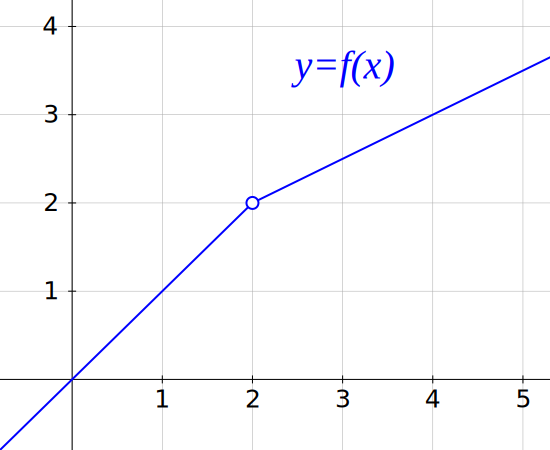
\includegraphics[scale=.3]{G3}
\end{center}
\begin{enumerate}
\item Find one value of $\delta>0$ s.t. \hfill \DS{0 < |x-2| < \delta \implies |f(x) - 2| < 0.5}
\item Find \emph{all} values of $\delta>0$ s.t. \hfill \DS{0 < |x-2| < \delta \implies |f(x) - 2| < 0.5}
\end{enumerate}



\end{frame}
%-----------------------
\begin{frame}
\frametitle{Warm-up}

Write down the formal definition of 
	$$
		\lim_{x \to a} f(x) = L.
	$$
\end{frame}

%-----------------------------
\begin{frame}
\frametitle{Side limits}

\begin{block}{Recall}
Let $L, a \in \mathbb{R}$. \\
Let $f$ be a function defined at least on an interval around $a$, except possibly at $a$. \\
	$$
		\lim_{x \to a} f(x) = L
	$$
means 
	$$
		\forall \varepsilon >0, \exists \delta >0 \mbox{ s.t. } \quad 0<|x-a|<\delta \implies |f(x)-L| < \varepsilon.
	$$
\end{block}

\vfill

Write, instead, the formal definition of 
	$$
		\lim_{x \to a^+} f(x) = L, \quad \mbox{ and } \quad \lim_{x \to a^-} f(x) = L.
	$$


\end{frame}
%-----------------------
\begin{frame}
\frametitle{Infinite limits}

\begin{block}{Definition}
Let $a \in \mathbb{R}$. \\
Let $f$ be a function defined at least on an interval around $a$, except possibly at $a$. \\
Write a formal definition for
	$$
		\lim_{x \to a} f(x) = \infty.
	$$
\end{block}

\end{frame}
%-----------------------
\begin{frame}[t]
\frametitle{Infinite limits - 2}

Which one(s) is the definition of \DS{\lim_{x \to a} f(x) = \infty } ?
\vfill
\begin{enumerate}
	\item \DS{\forall M \in \R, \, \exists \delta > 0 \; \mbox{ s.t. } 0 < |x-a|<\delta \; \implies \; f(x) > M}
	\vfill
	\item \DS{\forall M \in \Z, \, \exists \delta > 0 \; \mbox{ s.t. } 0 < |x-a|<\delta \; \implies \; f(x) > M}
	\vfill
	\item \DS{\forall M > 0, \, \exists \delta > 0 \; \mbox{ s.t. } 0 < |x-a|<\delta \; \implies \; f(x) > M}
	\vfill
	\item \DS{\forall M > 5, \, \exists \delta > 0 \; \mbox{ s.t. } 0 < |x-a|<\delta \; \implies \; f(x) > M}
	\vfill
%	\item \DS{\forall M \in \R, \, \exists \delta > 0 \; \mbox{ s.t. } |x-a|<\delta \; \implies \; f(x) \geq M}
%	\vfill
\end{enumerate}

\end{frame}
%-----------------------------
\begin{frame}[t]
\frametitle{Related implications}


Let $a \in \R$.  Let $f$ be a function.
Assume we know 
	$$
		0 < |x-a| < 0.1 \quad \implies \quad f(x) > 100
	$$
\vspace{-.5cm}
\begin{enumerate}
	\item  Which values of $M \in \R$ satisfy ... ?
		$$
			0 < |x-a| < 0.1 \quad \implies \quad f(x) > M \p
		$$
\vspace{-.5cm}
	\item  Which values of $\delta>0$ satisfy ... ?
		$$
				0 < |x-a| < \delta \quad \implies \quad f(x) > 100
		$$
\end{enumerate}	


\end{frame}
%-----------------------------
\begin{frame}
\frametitle{Strict or non-strict inequality?}

	Let $f$ be a function with domain $\R$.  One of these statements implies the other.  Which one?

\
	\begin{enumerate}
		\item  \DS{\forall M \in \R, \, \exists N \in \R \mbox{ s.t. }  x>N \implies f(x) > M}

\
		\item  \DS{\forall M \in \R, \, \exists N \in \R \mbox{ s.t. }  x>N \implies f(x) \geq M}
	\end{enumerate}


\end{frame}

%-----------------------------

\begin{frame}
\frametitle{Negation of conditionals}

Write the negation of these statements:
	\begin{enumerate}
		\item  If Justin Trudeau has a brother, then he also has a sister.
		\item  If a student in this class has a brother, then they also have a sister.
	\end{enumerate}	
\end{frame}

%-----------------------------
\begin{frame}
\frametitle{More negation}

Let $f$ be a function with domain $\mathbb{R}$.  Write the negation of the statement:
	\begin{equation*}
		\mbox{IF } \; 2<x<4, \quad \mbox{ THEN } \; 1<f(x)<3.  	
	\end{equation*}


\end{frame}

%-----------------------------
\begin{frame}
\frametitle{Existence}

Write down the formal definition of the following statements:

\vfill
\begin{enumerate}

\item  \DS{\lim_{x \to a} f(x) = L}
\vfill

\item  \DS{\lim_{x \to a} f(x) } exists

\vfill
\item  \DS{\lim_{x \to a} f(x) } does not exist

\end{enumerate}

\vfill

\end{frame}

%-----------------------
\begin{frame}[t]
\frametitle{Preparation: choosing deltas}

\begin{enumerate}
	\item  Find one value of $\delta >0$ such that  
		$$ |x-3|< \delta \implies |5x-15|<1.$$
	\item  Find \emph{all} values of $\delta >0$ such that  
		$$ |x-3|< \delta \implies |5x-15|<1. $$
	\item  Find \emph{all} values of $\delta >0$ such that  
		$$|x-3|< \delta \implies |5x-15|<0.1. $$
	\item  Let us fix $\e >0$.  Find \emph{all} values of $\delta >0$ such that  
		$$|x-3|< \delta \implies |5x-15|<\e.$$
\end{enumerate}

\end{frame}

%------------------------------

\begin{frame}
\frametitle{What is wrong with this ``proof"?}
\smallerfont
\vspace{-2mm}
\begin{block}{}%$\varepsilon-\delta$ Proofs}
Prove that 
$$
\lim_{x\to 3} (5x+1) = 16
$$
\end{block}

\begin{block}{``Proof:"}
	Let $\e>0$.

	WTS $\forall \e>0$, $\exists\delta>0$ s.t. 
		$$  0<|x-3|<\delta \implies |(5x+1) - (16)|<\e$$
\vspace{-3mm}
	\begin{align*}
		|(5x+1) - (16)|<\varepsilon &\iff |5x+15|<\e \\
		&\iff 5|x+3|<\e \implies\delta=\frac{\e}{3}
	\end{align*}
\hfill $\square$
\end{block}

\end{frame}


%-----------------------
\begin{frame}[t]
\frametitle{Your first $\e-\delta$ proof}

\begin{block}{Goal}
	We want to prove that
		\begin{equation} \label{eq:uno}
			\lim_{x \to 3} \left( 5x + 1 \right) = 16
		\end{equation}
	directly from the definition.
\end{block}
\vfill 
\begin{enumerate}
\p		\item  Write down the formal definition of the statement \eqref{eq:uno}.
\p		\item  Write down what the structure of the formal proof should be, without filling the details.
\p		\item  Write down a complete formal proof.
\end{enumerate}
\vfill
\end{frame}

%-----------------------------
\begin{frame}
\frametitle{A harder proof}

\begin{block}{Goal}
	We want to prove that
		\begin{equation} \label{eq:dos}
			\lim_{x \to 0} \left( x^3 + x^2 \right) = 0
		\end{equation}
	directly from the definition.
\end{block}
\vfill 
\begin{enumerate}
\pause	\item  Write down the formal definition of the statement \eqref{eq:dos}.
\pause	\item  Write down what the structure of the formal proof should be, without filling the details.
\pause	\item  Rough work:  What is $\delta?$
\pause	\item  Write down a complete formal proof.
\end{enumerate}
\vfill

\end{frame}
%-----------------------------
\begin{frame}[t]
\frametitle{Is this proof correct?}

{\bf Claim:}
	$$
		\forall \e >0, \exists \delta>0 \mbox{ s.t. }  \quad 0<|x|<\delta \; \implies \;  |x^3+x^2| < \e.
	$$
\vfill
\begin{block}{Proof:}
	\begin{itemize}
		\item  Let $\e >0$.
		\item  Take \DS{\delta = \sqrt{\frac{\e}{|x+1|}}}.
		\item Let $x \in \R$.  Assume $0 < |x| < \delta$.  Then
			$$
				|x^3+x^2| = x^2 | x + 1| < \delta^2 |x+1| = \frac{\e}{|x+1|} |x+1| = \e.
			$$
		\item	 I have proven that \DS{|x^3+x^2| < \e}. 
		\hfill \qed
	\end{itemize}
\end{block}

\vfill

\end{frame}

%-----------------------
\begin{frame}[t]
\frametitle{Choosing deltas again} 

Let us fix numbers $A, \e >0$.  Find:

\vfill

\begin{enumerate}
	\item  a value of $\delta >0$ \; s.t.  \hfill \DS{|x|< \delta \implies |Ax^2|<\e}
\p \vfill
	\item  \emph{all} values of $\delta >0$ \; s.t.  \hfill \DS{|x|< \delta \implies |Ax^2|<\e}
\p \vfill
	\item a value of $\delta >0$ \; s.t.   \hfill \DS{|x|< \delta \implies |x+1| < 10}
\p \vfill
	\item \emph{all} values of $\delta >0$ \; s.t.   \hfill \DS{|x|< \delta \implies |x+1| < 10}
\p \vfill
	\item a value of $\delta >0$  \; s.t.   \hfill \DS{|x|< \delta \implies \left\{  \begin{array}{c} |Ax^2|<\e \\ |x+1| < 10 \end{array} \right. }
\p \vfill
	\item a value of $\delta >0$ \; s.t. \hfill \DS{|x| < \delta \implies |(x+1)x^2| < \e }
\vfill
\end{enumerate}

\end{frame}

%-----------------------
\begin{frame}[t]
\frametitle{Indeterminate form}


Let $a \in \R$. 
Let $f$ and $g$ be positive functions defined near $a$, except maybe at $a$. 

\vfill

Assume 
	\DS{
		\lim_{x \to a} f(x) = \lim_{x \to a} g(x) = 0
	}.

\vfill

What can we conclude about  \quad
	\DS{
		\lim_{x \to a} \frac{f(x)}{g(x)} 
	} ?

\vfill

\begin{multicols}{2}
\begin{enumerate}
	\item The limit is $1$.
	\item The limit is $0$.
	\item The limit is $\infty$.
	\item The limit does not exist.
	\item  We do not have enough information to decide.
\end{enumerate}
\end{multicols}

\end{frame}

%-----------------------
\begin{frame}
\frametitle{A theorem about limits}
\smallerfont
\begin{block}{}
 Let $f$ be a function with domain $\R$ such that 
$$
\lim_{x\to 0} f(x) = 3
$$
Prove that 
$$
\lim_{x\to 0} \left[  5 f(2x) \right] =15
$$
directly from the definition of limit.  Do not use any of the limit laws.
\end{block}
\begin{enumerate}
\pause	\item  Write down the formal definition of the statement you want to prove.
\pause	\item  Write down what the structure of the formal proof should be, without filling the details.
\pause	\item  Rough work.
\pause 	\item  Write down a complete proof.
\end{enumerate}

\end{frame}
%-----------------------------
\begin{frame}[t]
\frametitle{Proof feedback}

\begin{enumerate}
	\item  Is the structure of the proof correct?  \\
	(First fix $\e$, then choose $\delta$, then ...)
	\item  Did you say exactly what $\delta$ is?
	\item  Is the proof self-contained?  \\
	 (I do not need to read the rough work)
	\item  Are all variables defined?  In the right order? 
	\item  Do all steps follow logically from what comes before? \\
	Do you start from what you know and prove what you have to prove? \\
	\item  Are you proving your conclusion or assuming it?
\end{enumerate}


\end{frame}
%-----------------------
\begin{frame}[t]
\frametitle{A new squeeze}
\smallerfont
This is the Squeeze Theorem, as you know it:

\begin{block}{The (classical) Squeeze Theorem}
	Let $a, L \in \R$. \\
	Let $f$, $g$, and $h$ be functions defined near $a$, except possibly at $a$.

\vspace{.2cm}
	\begin{tabular}{cl}
		IF  & $\bullet$ {For $x$ close to $a$ but not $a$,} \;
			 \DS{
			 h(x) \leq g(x) \leq f(x)
			 } 
			 \\ \vspace{-0.2cm} \\
		&  $\bullet$  \DS{\lim_{x \to a} f(x) = L} \quad and
				\quad\DS{ \lim_{x \to a} h(x) = L } \\ 
		\vspace{-.1cm} \\
		THEN & $\bullet$ \DS{\lim_{x \to a} g(x) = L}
	\end{tabular}
\end{block}

\pause
Come up with a new version of the theorem about limits being infinity.    
(The conclusion should be \DS{\lim_{x \to a} g(x) = \infty}.)

\

\emph{Hint:}  Draw a picture for the classical Squeeze Theorem.  Then draw a picture for the new theorem. 

\end{frame}
%-----------------------
\begin{frame}[t]
\frametitle{A new squeeze}
\smallerfont
\begin{block}{The (new) Squeeze Theorem}
	Let $a \in \R$. \\
	Let $g$ and $h$ be functions defined near $a$, except possibly at $a$.

\vspace{.2cm}
	\begin{tabular}{cl}
		IF  & $\bullet$ {For $x$ close to $a$ but not $a$,} \;
			 \DS{%\exists p >0, \mbox{ s.t. } 0 < |x-a| < p \; \implies \; 
			 h(x) \leq g(x) 
			 } 
			 \\ \vspace{-.2cm} \\
		&    $\bullet$ \DS{ \lim_{x \to a} h(x) = \infty } \\ 
		\vspace{-.1cm} \\
		THEN & $\bullet$ \DS{\lim_{x \to a} g(x) = \infty}
	\end{tabular}
\end{block}

\begin{enumerate}
\p
	\item  Replace the first hypothesis with a more precise mathematical statement.
\p
	\item  Write down the definition of what you want to prove.
\p
	\item  Write down the structure of the formal proof.
\p
	\item  Rough work
\p
	\item  Write down a complete, formal proof.
\end{enumerate}
\end{frame}
%-----------------------
\begin{frame}
\frametitle{True or False?}

\vfill

Is this theorem true?

\vfill

\begin{block}{Claim}
Let $a \in \R$. \\
Let $f$ and $g$ be functions defined near $a$. \\
\begin{itemize}
	\item IF \DS{\lim_{x \to a} f(x) = 0},
	\item  THEN \DS{\lim_{x \to a} \left[ f(x) g(x) \right] = 0}.
\end{itemize}
\end{block}

\vfill

\end{frame}
%-----------------------------
\begin{frame}[t]
\frametitle{A new theorem about products}
\smallerfont
\begin{block}{Theorem}
Let $a \in \R$.  Let $f$ and $g$ be functions with domain $\R$, except possibly $a$. 
 Assume
	\begin{itemize}
		\item  \DS{\lim_{x \to a} f(x) = 0}, and
		\item $g$ is bounded. 
			This means that 
			$$\exists M >0 \mbox{ s.t. } \forall x \neq a, |g(x)| \leq M.$$
	\end{itemize}
THEN  \DS{\lim_{x \to a} \left[ f(x) g(x) \right] = 0}
\end{block}

 \vfill 
\begin{enumerate}
\p	\item  Write down the formal definition of what you want to prove.
\p	\item  Write down what the structure of the formal proof.
\p 	\item  Rough work.
\p	\item  Write down a complete formal proof.
\end{enumerate}
\vfill

\end{frame}
%-----------------------------
\begin{frame}[t]
\frametitle{Critique this ``proof" -- \#1}
\smallerfont
\begin{itemize}
	\item  WTS \DS{\lim_{x \to a} \left[ f(x) g(x) \right] = 0}:
	
		\hfill \DS{\forall \e>0, \exists \delta>0} \; s.t. \; \DS{0<|x-a|<\delta \implies \azul{|f(x) g(x)| < \e}}. 
\vfill	
	\item  We know \DS{\lim_{x \to a} f(x) = 0}
	
		\hfill \DS{\forall \e_1>0, \exists \delta_1 >0 } \; s.t. \; \DS{0<|x-a|<\delta_1 \implies \azul{|f(x)| <\e_1}}.
\vfill
	\item   We know \hfill \DS{\exists M>0} \; s.t. \; \DS{\forall x \neq 0, \; \; \azul{|g(x)| \leq M}}.
\vfill
	\item  \DS{|f(x)g(x)| = |f(x)||g(x)| < \e_1 M}
\vfill
	\item \DS{\e = \e_1 M \implies \e_1 = \frac{\e}{M}}
\vfill
	\item Take  \DS{\delta = \delta_1}
\vfill
\end{itemize}
\end{frame}

%-----------------------------
\begin{frame}[t]
\frametitle{Critique this ``proof" -- \#2}
\smallerfont
\begin{itemize}
	\item  WTS \DS{\lim_{x \to a} \left[f(x) g(x) \right] =0}.  By definition, WTS:
	
		\hfill \DS{\forall \e>0, \exists \delta>0} s.t. \DS{0<|x-a|<\delta \implies |f(x) g(x)|<\e }
\vfill
	\item  Let $\e >0$.  
\vfill
	\item Use the value \DS{\frac{\e}{M}} as ``epsilon" in the definition of \DS{\lim_{x \to a} f(x) = 0}
		
		\hfill  \DS{\exists \delta_1 \in \R} s.t. \DS{0<|x-a|<\delta_1 \implies |f(x)| <  \frac{\e}{M} }.
\vfill
	\item Take \DS{\delta = \delta_1}.
\vfill
	\item  Let \DS{x \in \R}.  Assume \DS{0 < |x-a| <\delta}
\vfill
	\item  Since \DS{\exists M>0} s.t. \DS{\forall x \neq 0, |g(x)| \leq M} \\
		\hfill \DS{|f(x) g(x)| < \frac{\e}{M} \cdot M = \e}.
\vfill
\end{itemize}

\end{frame}

%-----------------------------
\begin{frame}[t]
\frametitle{Critique this ``proof" -- \#3}
\smallerfont
\begin{itemize}
	\item  Since $g$ is bounded, \DS{\exists M >0} \; s.t. \; \;\DS{\forall x \neq 0, \; |g(x)| \leq M}
\vfill
	\item  Since \DS{\lim_{x \to a} f(x)=0}, there exists \DS{\delta_1 >0} s.t. 
	
		if \DS{0<|x-a|<\delta_1}, \quad then \; \DS{|f(x)-0| = |f(x)| <\e_1 = \frac{\e}{M}}.
\vfill
	\item \ \vspace{-1cm}
		$$ 
			|f(x)g(x)| = |f(x)| \cdot |g(x)| \leq |f(x)| \cdot M < \e_1 \cdot M = \frac{\e}{M} \cdot M = \e
		$$
	\item  In summary, by setting \DS{\delta = \min\{\delta_1 \}}, we find that
	
	\
	
	if \DS{0<|x-a|<\delta}, \quad then \; \DS{|f(x) \cdot g(x)| < \e}.
\vfill
\end{itemize}
\end{frame}

%-----------------------------

\begin{frame}
\frametitle{Limits involving \DS{\sin(1/x)} Part I}

\begin{block}{
The reason that \DS{{\lim_{x\rightarrow 0}\sin (1/x)}} does not exist is:}

\begin{enumerate}
\item because the function values oscillate around $0$
\item because $1/0$ is undefined
\item because no matter how close $x$ gets to $0$, there are $x$'s near $0$ for which $\sin(1/x) =1$, and some for which $\sin (1/x)=-1$
\item all of the above
\end{enumerate}

\end{block}

\end{frame}


%-----------------------------

\begin{frame}
\frametitle{Limits involving \DS{\sin(1/x)} Part II}

\begin{block}{The limit 
$\displaystyle{\lim_{x\rightarrow 0}x^2\sin (1/x)}$ }
\begin{enumerate}
\item does not exist because the function values oscillate around $0$
\item does not exist because $1/0$ is undefined
\item does not exist because no matter how close $x$ gets to $0$, there are $x$'s near $0$ for which $\sin(1/x) =1$, and some for which $\sin (1/x)=-1$
\item equals 0 
\item equals 1
\end{enumerate}
\end{block}
\end{frame}


%-----------------------------

\begin{frame}
\frametitle{Absolute value and the Squeeze Theorem}

Use the Squeeze Theorem to prove:
\begin{theorem}
IF \DS{\lim_{x\to a}|f(x)| = 0}, THEN \DS{\lim_{x\to a}f(x)=0}.\\
\end{theorem}

\

\emph{Hint:} Recall that $-|c| \leq c \leq |c|$ for every $c \in \R$.

\end{frame}

%-----------------------------
\begin{frame}[t]
\frametitle{Undefined function}
\smallerfont
Let $a \in \R$ and let $f$ be a function.   Assume $f(a)$ is undefined.

\vfill

\begin{block}{What can we conclude?}
	\begin{enumerate}
		\item  \DS{\lim_{x \to a} f(x)} exist
		\item  \DS{\lim_{x \to a} f(x)} doesn't exist.
		\item   No conclusion.  \DS{\lim_{x \to a} f(x)} may or may not exist.
	\end{enumerate}
\end{block}

\vfill

\begin{block}{What else can we conclude?}
	\begin{enumerate} \addtocounter{enumi}{3}
		\item  $f$ is continuous at $a$.
		\item  $f$ is not continuous at $a$.
		\item  No conclusion. $f$ may or may not be continuous at $a$.
	\end{enumerate}
\end{block}

\vfill
	
\end{frame}

%-----------------------------
\begin{frame}
\frametitle{A new function}

\begin{itemize}
\item Let $x, y \in \R$.  What does the following expression calculate?  Prove it.
	$$
		f(x,y) = \frac{x + y + |x - y|}{2}
	$$
\emph{Suggestion:}  If you don't know how to start, try some sample values of $x$ and $y$.
\vfill  \p

\item Write a similar expression to compute \DS{\min \{ x, y \}}.
\end{itemize}
\vfill

\end{frame}
%-----------------------------
\begin{frame}
\frametitle{More continuous functions}

We want to prove the following theorem
\begin{block}{Theorem}
IF $f$ and $g$ are continuous functions \\
THEN $h(x) = \max \{ f(x), g(x) \}$ is also a continuous function.
\end{block}

You are allowed to use all results that we already know.  What is the fastest way to prove this?


\vfill


\emph{Hint:}  
There is a way to prove this quickly without writing any epsilons.

\vfill

\end{frame}

%------------------------------
\begin{frame}
\frametitle{True or False? -- Discontinuities}

	\begin{enumerate}
		\item IF $f$ and $g$ have removable discontinuities at $a$
		
			THEN  $f+g$ has a removable discontinuity at $a$
		
		\
		\item IF $f$ and $g$ have non-removable discontinuities at $a$
		
			THEN $f+g$ has a non-removable discontinuity at $a$
	\end{enumerate}


\end{frame}
%------------------------------
\begin{frame}
\frametitle{Which one is the correct claim?}


\begin{block}{Claim 1?}
(Assuming these limits exist)
$$
	\lim_{x \to a} g(f(x))  \; = \; g \left(  \lim_{x \to a} f(x) \right)
$$
\end{block}

\vfill

\begin{block}{Claim 2?}
\begin{tabular}{lll}
	IF 
		&
	\azul{(A)} \DS{\lim_{x \to a} f(x) = L}, \quad and
		&
	\azul{(B)} \DS{\lim_{t \to L} g(t) = M \ }
		\\
	THEN
		&
	\azul{(C)} \DS{\lim_{x \to a} g(f(x)) =   M \; }
\end{tabular}
\end{block}


\end{frame}
%------------------------------
\begin{frame}
\frametitle{A difficult example}

Construct a pair of functions $f$ and $g$ such that
	\begin{align*}
		\lim_{x \to 0} f(x) \; & \; = \; 1  \\
		\lim_{t \to 1} g(t) \; & \; = \; 2 \\
		\lim_{x \to 0} g(f(x)) \; & \; = \; 42
	\end{align*}

\end{frame}
%------------------------------
\begin{frame}
\frametitle{Transforming limits}

The only thing we know about the function $g$ is that
	$$
		\lim_{x \to 0} \frac{g(x)}{x^2} = 2.
	$$
Use it to compute the following limits:

	\begin{multicols}{2}
	\begin{enumerate}	
		\item \DS{\lim_{x \to 0} \frac{g(x)}{x}}  				
		\item \DS{\lim_{x \to 0} \frac{g(x)}{x^4}} 					
		\item \DS{\lim_{x \to 0} \frac{g(3x)}{x^2}}  	
	\end{enumerate}
	\end{multicols}
	
\end{frame}
%------------------------------
\begin{frame}
\frametitle{Limits at infinity}

Compute:

\begin{enumerate}
\begin{multicols}{2}
	\item \DS{\lim_{x \to \infty} \left(x^7-2x^5+11\right)}
	\item \DS{\lim_{x \to \infty} \left(x^2 - \sqrt{x^5+1} \right)}
	\item \DS{\lim_{x \to \infty} \frac{x^2+11}{x+1}}
	\item \DS{\lim_{x \to \infty} \frac{x^2+2x+3}{3x^2+4x+5}}
	
	\
	
	\item \DS{\lim_{x \to \infty} \frac{x^3 + \sqrt{2x^6+1}}{2x^3+ \sqrt{x^5+1}}}
\end{multicols}
\end{enumerate}

\end{frame}
%------------------------------
\begin{frame}
\frametitle{Trig computations}

Using that \DS{\lim_{x \to 0} \frac{\sin x}{x} = 1}, compute the following limits:

\

\begin{enumerate}
\begin{multicols}{2}
	\item \DS{\lim_{x \to 2} \frac{\sin x}{x} }
	\item \DS{\lim_{x \to 0} \frac{\sin (5x)}{x} }
	\item \DS{\lim_{x \to 0} \frac{\tan^2 (2x^2)}{ x^4} }
	\item \DS{\lim_{x \to 0} \frac{\sin e^x}{e^x} }
	\item \DS{\lim_{x \to 0} \frac{1 - \cos x}{x} }
	\item \DS{\lim_{x \to 0}  \frac{\tan^{10}(2x^{20})}{\sin^{200}(3x)} }
\end{multicols}
\p
	\item  \ \vspace{-.6cm}
	
	{\smallerfont \DS{\lim_{x \to 0} \left[  (\sin x) \; (\cos (2x)) \; (\tan (3x)) \; (\sec (4x) ) \; (\csc (5x)) \; (\cot (6x)) \right]} }
\end{enumerate}

\end{frame}
%------------------------------
\begin{frame}
\frametitle{Plus or minus infinity?}

Compute:
\begin{enumerate}
\begin{multicols}{2}
	\item  \DS{\lim_{x \to -3^+} \;  \frac{x^2-9}{3-2x-x^2}}

	\item  \DS{\lim_{x \to 1^+} \; \frac{x^2-9}{3-2x-x^2}}
\end{multicols}
\end{enumerate}

\end{frame}
%-----------------------------
\begin{frame}
\frametitle{A harder limit}

Calculate

	$$
		\lim_{x \to 2} \frac{\left[\sqrt{2+x} -2\right] \left[ \sqrt{3+x} - 3 \right]}{\sqrt{x-1} - 1}
	$$

\end{frame}
%-----------------------------
\begin{frame}
\setsize{13}
\frametitle{Which solution is right?}
Compute \DS{L = \lim_{x \to -\infty} \left[  x - \sqrt{x^2+x} \right]}.

\begin{itemize}
	\item {\bf Solution 1}
{\setsize{11}
		\begin{align*}
			L = & \lim_{x\to -\infty} \frac{\left[  x - \sqrt{x^2+x} \right] \; \left[  x + \sqrt{x^2+x} \right]}{\left[  x + \sqrt{x^2+x} \right]}
			= \lim_{x \to -\infty} \frac{x^2-(x^2+x)}{\left[  x + \sqrt{x^2+x} \right]}
				\\
			=& \lim_{x \to -\infty}\frac{-x}{x \left[ 1 + \sqrt{1 + \frac{1}{x}} \right]} 
			= \lim_{x \to -\infty}\frac{-1}{ \left[ 1 + \sqrt{1 + \frac{1}{x}} \right]}
			= \frac{-1}{2}
		\end{align*}	
}
	\item  {\bf Solution 2}
		$$
			L = \lim_{x \to -\infty} \left[ {\color{red} x }- {\color{blue} \sqrt{x^2+x} }\right] = {\color{red}(-\infty)} - {\color{blue}\infty} = - \infty
		$$
\end{itemize}

\end{frame}
%-----------------------------
\begin{frame}
\frametitle{Can we conclude this?}

\begin{itemize}
	\item Consider the function \DS{(x)=\frac{4}{x}}.
\vfill
	\item We have \quad $f(-1)=-4<0$  \quad and \quad $f(1)=4>0$. 
\vfill
	\item Use IVT.
	
	 Can we conclude $f(c)=0$ for some $c\in(-1,1)$?
\end{itemize}
\vfill \vfill

\end{frame}

%-----------------------------
\begin{frame}
\frametitle{Existence of solutions}

Prove that the equation 
	$$
		x^4 - 2x = 100
	$$
has at least two solutions.

\end{frame}
%-----------------------------
\begin{frame}[t]
\frametitle{Can this be proven? (Use IVT)}
\smallerfont
\begin{enumerate}
\item  Prove that there exists a time of the day when the hour hand and the minute hand of a clock form an angle of exactly 23 degrees.

\p \vfill
\item  During a Raptors basketball game, at half time the Raptors have 52 points.  Prove that at some point they had exactly 26 points.

\p \vfill
\item  Prove that at some point during Alfonso's life, his height in centimetres was exactly equal to 10 times his weight in kilograms.  Some data:
	\begin{itemize}
		\item  His height at birth: 47 cm
		\item  His weight at birth: 3.2 kg
		\item  His height today: 172 cm
	\end{itemize}
\vfill
\end{enumerate}

\end{frame}

%-----------------------------
\begin{frame}
\frametitle{Temperature}
	
	On June 09, 2016, the outside temperature in Toronto at 6 AM was $10^\circ$. At 4 PM,
the temperature was $20^\circ$. 

\begin{enumerate}


\item Must there have been a time between 6 AM and 4 PM when the temperature was $15^\circ$?
Explain how you know. Which assumption about temperature allows you to reach your conclusion?


\item Must there have been a time between 6 AM and 4 PM when the temperature was $22^\circ$?
Explain how you know.


\item Could there have been a time between 6 AM and 4 PM when the temperature was $22^\circ$?
Explain how you know.

\end{enumerate}
\end{frame}

%-----------------------------
\begin{frame}
\frametitle{Extrema}

In each of the following cases, does the function $f$ have a maximum and a minimum on the interval $I$?

\

\begin{enumerate}
	\item  \DS{f(x) = x^2}, \quad \DS{I = (-1,1)}.
	\item   \DS{f(x) = \frac{(e^x + 2) \sin x}{x} - \cos x + 3 }, \quad  \DS{I = [2,6]}
	\item   \DS{f(x) = \frac{(e^x + 2) \sin x}{x} - \cos x + 3 }, \quad  \DS{I = (0,5]}
\end{enumerate}



\end{frame}
%-----------------------------
\begin{frame}
\frametitle{Definition of maximum}

Let $f$ be a function with domain $I$.  \\
Which one (or ones) of the following is (or are) a definition of 	\quad
	``$f$ has a maximum on $I$"?

\begin{enumerate}
	\item   \DS{\forall x \in I}, \DS{\exists C \in \R} s.t. \DS{f(x) \leq C}
	\item  \DS{\exists C \in I} s.t. \DS{\forall x \in I}, \DS{f(x) \leq C}
	\item  \DS{\exists C \in \R} s.t. \DS{\forall x \in I}, \DS{f(x) \leq C}
	\item  \DS{\exists C \in \R} s.t. \DS{\forall x \in I}, \DS{f(x) < C}
\end{enumerate}

\end{frame}
%-----------------------------
\begin{frame}
\frametitle{More on the definition of maximum}


Let $f$ be a function with domain $I$.  \\
What does each of the following mean?

\begin{enumerate}
	\item  \DS{\exists C \in \R} s.t. \DS{\forall x \in I}, \DS{f(x) \leq C}
	\item  \DS{\exists C \in \R} s.t. \DS{\forall x \in I}, \DS{f(x) < C}
	\item  \DS{\exists a \in I} s.t. \DS{\forall x \in I}, \DS{f(x) \leq f(a)}
	\item  \DS{\exists a \in I} s.t. \DS{\forall x \in I}, \DS{f(x) < f(a)}
\end{enumerate}

\end{frame}


%-----------------------------
%-----------------------------
\end{document}
%-----------------------------
%-----------------------------
%-----------------------------









